%!TEX root = ../report.tex

% 
% Architecture
% 

% 2/3 pages
%Your proposed architecture. Can have lots of pictures and 
% bullet points so it is easy to understand.
\section{Architecture}
\label{sec:architecture}
We propose a framework to develop mobile web apps for smart
places, that allow developers to only write the code
for the application logic and the specific behavior when
the user is nearby specific points of interest (POI).
Each beacon represents one POI. Developers will not need
to write the code that gets beacons' data and get the
right information from a backend. They will need only
to write the code for each specific POI. They could give
a name to each POI and the app will receive that name 
instead of the beacon's raw data. 

One of the main goals of this project is to allow
users to interact with any Smart Place, without
the need to install one native app for each one.
Mobile web apps do not need to be installed because
they run in the device's browser.
This is the main reason why our framework will
target mobile web apps instead of native ones.
This means that, when the user starts to interact
with a Smart Place, he will initially discover the
beacons using a native app but from that moment
onwards
he will interact with a mobile
web app, running in his mobile device's browser.

However, detecting
nearby beacons is not a feature integrated in the mobile
Operating System. Our solution would be to build the
Smart Places App,
that detects nearby beacons, turn them into names and
other high-level information, and deliver it to the
mobile web app. The user would need only this app to
be able to access any smart place app. Also, the same app
could be used to configure a smart place.
Considering the restaurant example, mentioned in
\ref{sub:bluetooth_low_energy}, some
developers, could develop the app for restaurants,
using our framework. These developers would only think
about tables instead of beacons. The owner would need
to put a beacon in each table. After the beacons
installation, he could just use the Smart Places App,
choose the app for restaurants, and put his smartphone
closer to a beacon and configure it. This configuration
would be, for each beacon, what is the number of the table
where it is deployed. Then, his customers would only
need the Smart Places App, turn on bluetooth and they will
be notified that they can make their orders from their
smartphones.

%Solution overview
Our solution has three main components,
the BLE Beacons, as it is shown in Figure 
\ref{fig:overview_architecture}, 
the Backend and an Android app
that will run on the users' smartphones.
\begin{figure}[!ht]
  \centering
    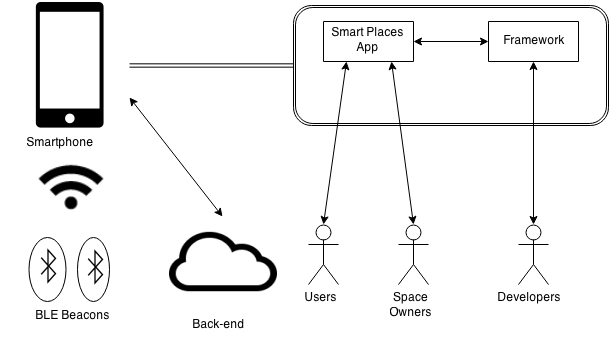
\includegraphics[width=0.9\textwidth]{img/overview_architecture}
    \caption{Overview of the proposed solution}
    \label{fig:overview_architecture}
\end{figure}
The \textbf{BLE Beacons}, as explained in section 
\ref{sec:introduction}, are small devices that broadcast
an ID using Bluetooth Low Energy. The \textbf{Backend} is where information about each beacon is stored. 
And, the users'
\textbf{smartphones}, is where the 
\textbf{Smart Places App} will run.
It is a native Android app that will scan for 
nearby beacons,
get the information about them from the Backend and
provide that information to the app associated to a 
given Smart Place.
\textbf{Users} will use this app to have access
to any app running in any Smart Place.
Also, \textbf{Smart Places Owners} can use it to configure
their Smart Places and configure which applications
will run there.
Since these apps will be mobile web apps, they will run
in a embedded web browser inside the Smart Places App.
\textbf{Developers} will need to use the \textbf{Framework} to
develop such apps. Also, the Framework will provide an
Interface between the mobile web app, that will run
in a given Smart Place, and the Smart Places App.

\subsection{Smart Places App}
\label{sub:smart_places_app}
Figure \ref{fig:architecture} shows the two main
blocks that will run inside the smartphone.
We have the Smart Places App and the Framework itself.
\begin{figure}[!ht]
  \centering
    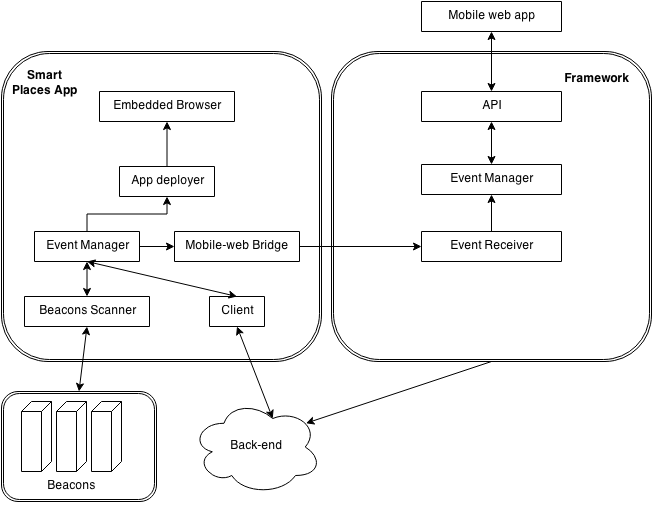
\includegraphics[width=0.9\textwidth]{img/architecture}
    \caption{Architecture}
    \label{fig:architecture}
\end{figure}
As already mentioned, the Smart Places App will be a native
Android app that the user and the Owner 
will use,
in order to be able to use any app of any Smart Place
and configure a Smart Place, respectively.
The \textbf{Beacons Scanner} will scan for nearby
beacons. After scanning, it will deliver the IDs
of the beacons to the \textbf{Beacons Manager}.
The Beacons Manager will call the \textbf{Client} to
get the information about each POI that is being
represented by each beacon from the backend or
from the \textbf{Beacons Cache}. It will be possible to
configure the Smart Places App to use the cache or not.
This cache will be an optimization to avoid communication
with the backend in each scan. If this cache is being
used, when a scan is completed, the Client will
check if the information about that beacon is in
the cache. If it is, the Client does not need to request
data from the backend. Otherwise, the Client will
request the information about all the POIs of that
Smart Place. In the next beacons scan, if we stay in
the same Smart Place, there is no need to make requests
to the backend since all the mapping between beacons
and POIs is in the cache.
After getting the POI information from the Client,
the Beacons Manager will call the \textbf{Mobile-web Bridge},
which provides an interface between the native app
and the web app, that will deliver this information
to the mobile web app that is running in the
\textbf{Embedded Web Browser}. 
Each time the web app needs to interact
with the native app, this component is called.
The \textbf{User Manager} is called to login the
user and to get the information about the user. 
To perform the user's login, the User Manager
will call the Client that will send the needed information
to the backend to login the user. After this step,
the mobile web app, can use the Mobile-web bridge
to get information about the logged in user.
The \textbf{Notification Service} is called to
show notifications in the user's mobile device.

\subsection{Framework}
\label{sub:framework}
The Framework provides, to developers, an \textbf{API} that they
can use to perform operations about the POIs or about the users.
Developers are allowed to define callbacks for each POI or to
even create new POIs. In order to do this, the API
uses the \textbf{POIs Manager} that will store the callbacks
for each POI.

In order to understand how the presented components
interact with each other and how the whole solution will
work, we need to take into consideration the data model
shown in Figure \ref{fig:uml}.
As mentioned in \ref{sec:introduction}, a Smart Place
is a set of POIs. Each BLE Beacon represents a POI.
Each POI has a name and a set of parameters, which are
pairs with a key and a value.
For instance, in the example of the restaurant,
introduced in section \ref{sub:bluetooth_low_energy},
each POI could have the name ``table'' and one 
parameter with key ``number'' and the value would
be the number of the table. Since the applications
that will belong to a Smart Place will be
mobile web apps, they will run in some web
server. This is why each Smart Place has an URL,
that will act as an entry point.

\begin{figure}[!ht]
  \centering
    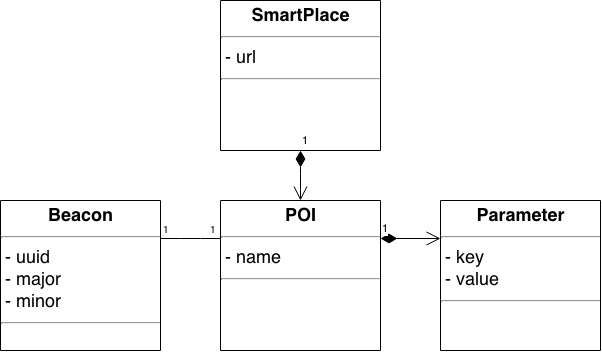
\includegraphics[width=0.9\textwidth]{img/smart-places-uml}
    \caption{Data Model}
    \label{fig:uml}
\end{figure}

% Two phases: Finding Smart Places and finding POIs
% First phase: how it works
% Second phase: how it works
% why two phases (this is not a CMS for beacons...
% more powerful...)
% Developers will only deal with POIs...

The mobile app that will be developed, 
the Smart Places App, will run in background,
scanning for nearby beacons. After the scan process,
if there are beacons that were found each one
can be mapped to one of the following kinds of
objects: Smart Place or POI.
Two phases can be considered: Finding Smart Places
and finding POIs.
As mentioned before, a Smart Place is a set of
POIs. Considering these two phases, the mobile app
will work as follows:

\begin{itemize}
\item After beacons are found, the app will try to map
these beacons to Smart Places. Figure
\ref{fig:sequence-smart-places} shows how the components
of the solution interact with each other to get
available Smart Places from the beacons that were found.
The Beacons Manager sends the list of found beacons
to the Client which will request, to the Backend,
to map those beacons to Smart Places.
After this step, the Beacons Manager calls the
Notification Service in order to show a notification
about the Smart Places that were found.
Then, the user can ignore the notification or
choose one Smart Place. If he selects one,
the Beacons Manager calls the Mobile-Web Bridge,
which will request the Embedded Web Browser to load
the URL of the selected Smart Place. Now, the user
will have access to the web application associated
with the Smart Place;
\item In the same Smart Place, the user will
pass near multiple POIs. The process of mapping
beacons to POIs is shown in Figure
\ref{fig:sequence-poi}.
After the previous
phase, the app will keep running in background
scanning for beacons. However, after beacons
are found, the Beacons Manager will select the
nearest beacon, that belongs to the Smart Place
that the user selected. Then, the Beacons
Manager calls the Client that will request
the Backend to get the POI object for that
beacon. After the Client receives the response,
it is sent back to the Beacons Manager, which will
call the Notification Service to show a notification,
in the user's mobile device, about the POI that was
found. After the user clicks on the notification,
the Beacons Manager will call the Mobile-Web
Bridge to deliver the POI object to the mobile
web application that belongs to the Smart Place
and is running in the Embedded Web Browser.
\end{itemize}

\begin{figure}[!ht]
  \centering
    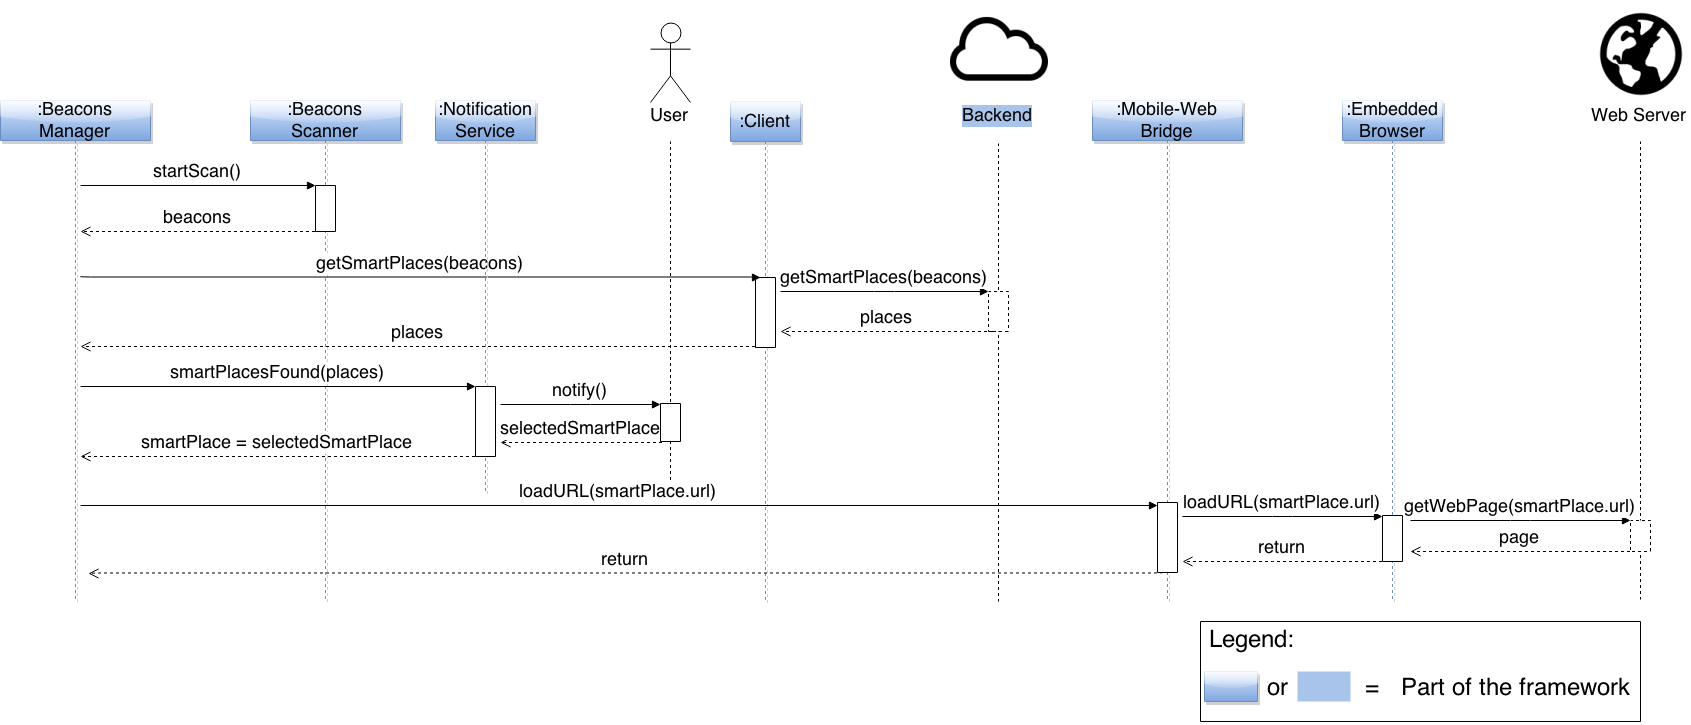
\includegraphics[width=1\textwidth]{img/smart-places-sequence}
    \caption{Discover smart place sequence diagram}
    \label{fig:sequence-smart-places}
\end{figure}

\begin{figure}[!ht]
  \centering
    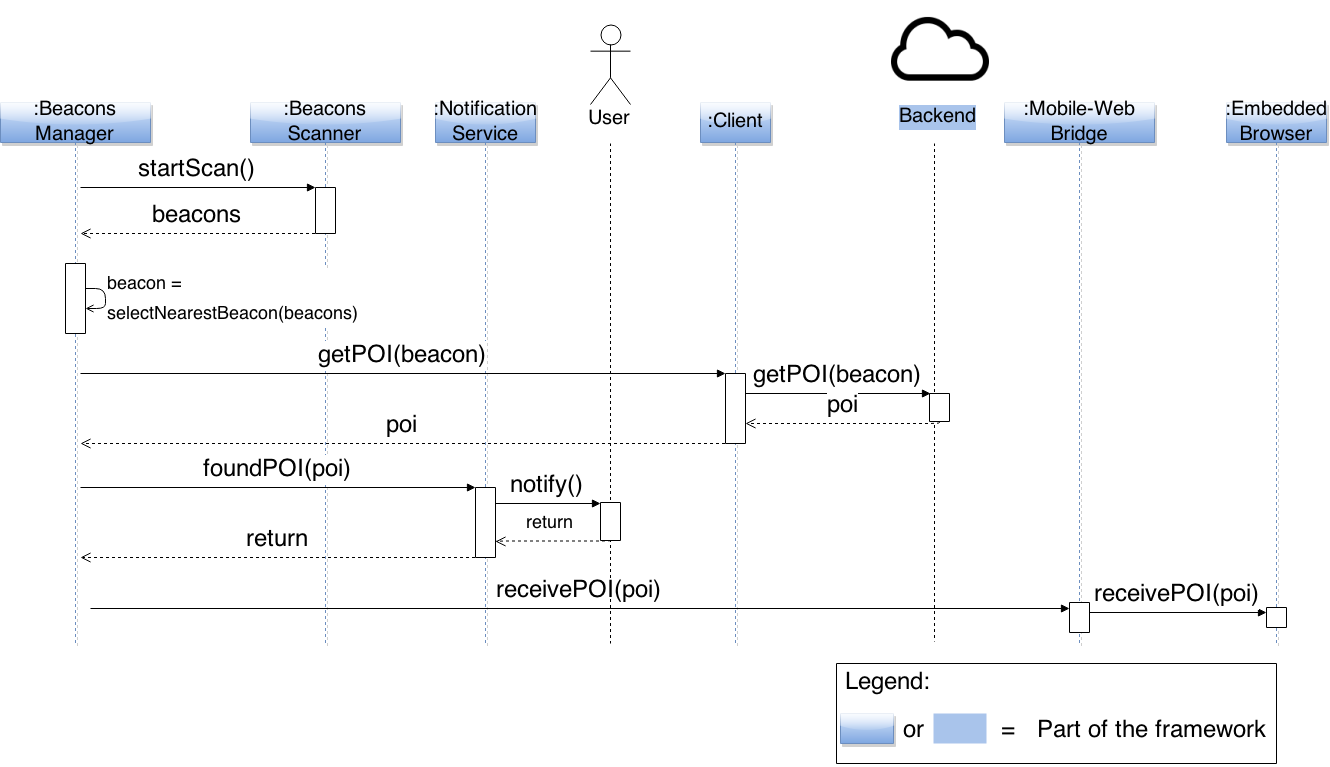
\includegraphics[width=1\textwidth]{img/smart-places-poi-sequence}
    \caption{Mapping beacons in a smart place sequence diagram}
    \label{fig:sequence-poi}
\end{figure}

As mentioned before, all the mapping between
beacons and Smart Places and POIs will be handled
by the framework. Developers will be able
to develop their applications without having to
configure any backend and writing code to handle
the BLE Beacons.
They will only write the code
that will run inside the Embedded Web Browser.
Their applications will receive POI objects,
which can be handled by any function. Since
these functions will run in the mobile
device's browser sandbox there are no security
issues about any malicious code.

In terms of development of the framework there are
several technical challenges:
\begin{itemize}

\item The time interval, between each
scan process.
If this value is too high
some beacons can be missed and the user will
not be able to interact with some Smart Places.
If this value is too low, the user will run out
of battery faster than usual;

\item If the user is nearby a lot of Smart Places
too many notifications can appear in his mobile
device. A solution could be to put all
the Smart Places that were found in just one
notification. However, when the user moves more
beacons can be scanned and more Smart Places
will be discovered and the user will receive
more notifications;

\item Get the nearest beacon. As explained before,
when the user chose a Smart Place, the mobile
app will keep on running in background 
trying to map beacons to POIs. Only the
nearest beacon is selected in each scan.
Most beacons vendors provide SDKs to handle
scanning and getting information from the beacons.
Most of them allow developers to get the distance.
Unfortunately, the method used to get this
value is not so accurate because it relies on the strength
of the signal, which can be very weak due to
many factors besides the distance, since it
is a wireless signal.

\item How to pass POI objects from the mobile
app to the web application running inside the
Embedded Web Browser.
The application that belong to a Smart Place
will run in the mobile device's browser.
However, after mapping beacons to POI objects,
those objects need to be passed to the 
application in the browser. This objects
are acquired by the mobile app that runs
native code and need to be passed to
code that is running in the browser
that is typically Javascript and not native.

\end{itemize}

In section \ref{sub:summary} the main limitations 
of related work were presented.
The solution being proposed here tries to
circumvent them. The Smart Places App will
offer, to the owners of Smart Places, an interface
where they can manage their POIs.
In terms of communication with the backend,
REST\cite{richardson2008restful} will be used instead
of SOAP. To invoke SOAP web services the client needs
to get the specification from a 
WSDL\footnote{Web Services Description Language:
http://www.w3.org/TR/wsdl} file, specify the
transport protocol and encode the request in a
XML\footnote{Extensible Markup Language:
http://www.w3.org/XML/} document. To invoke a
RESTful web service the client just needs to know
the endpoints and make an 
HTTP\footnote{Hypertext Transfer Protocol:
http://tools.ietf.org/html/rfc7235} request.
If messages are encoding in 
JSON\footnote{JavaScript Object Notation:
http://www.json.org/}, they will
get smaller than if they were encoded in XML.
This is important to consider in a resource constrained
mobile environment. SOAP is more flexible than REST
because any transport protocol can be used and it is
possible to add headers to handle security features.
However, we do not need such flexibility.
Another limitation of related work is that developers
have to write code to interact with the technology
where location data comes from. Our solution aims to
create abstractions for the BLE Beacons, which is the
technology being used to get location data.
Our mobile app will scan for beacons and get all the
needed data from the backend. Developers will only have
to use POI objects instead of identifiers of beacons.
The mapping between beacons and POIs will be performed
by the framework.
In terms of permissions, our app will only need the
user to turn on the Bluetooth receiver of his
mobile device. He will not have to configure
anything else in order to use it.
To avoid to make the user install one native app
in order to be able to interact with a Smart Place
our solution will allow developers to develop their
applications for Smart Places using web technologies,
such as HTML, CSS and Javascript. This applications
will run in the Embedded Web Browser of our mobile app.
Also, instead of just mapping BLE Beacons to URLs we map
BLE Beacons to POI objects. Developers will receive
these objects, in their mobile web apps developed for
Smart Places, and any kind of computation can be 
performed instead of just redirecting the user to an
URL.
